\documentclass[11pt]{article}
\usepackage[utf8]{inputenc}	% Para caracteres en español
\usepackage{amsmath,amsthm,amsfonts,amssymb,amscd}
\usepackage{multirow,booktabs}
\usepackage[table]{xcolor}
\usepackage{fullpage}
\usepackage{lastpage}
\usepackage{enumitem}
%\usepackage[scale=0.97]{XCharter} %%%FONTNAME
\usepackage{fancyhdr}
\usepackage{mathrsfs}
\usepackage{wrapfig}
\linespread{1}%%%LINESPREAD
\usepackage{setspace}
\usepackage{calc}
\usepackage{multicol}
\usepackage{cancel}
\usepackage[retainorgcmds]{IEEEtrantools}
\usepackage[margin=3cm]{geometry}
\usepackage{amsmath}
\newlength{\tabcont}
\setlength{\parindent}{0.0in}
\setlength{\parskip}{0.05in}
\usepackage{empheq}
\usepackage{framed}
\usepackage[most]{tcolorbox}
\usepackage{xcolor}
\colorlet{shadecolor}{orange!15}
\parindent 0in
\parskip 12pt
\geometry{margin=1in, headsep=0.25in}
\theoremstyle{definition}
\newtheorem{defn}{Definition}
\newtheorem{reg}{Rule}
\newtheorem{exer}{Exercise}
\newtheorem{note}{Note}
\usepackage{hyperref}
\hypersetup{
    colorlinks=true,
    linkcolor=blue,
    filecolor=magenta,      
    urlcolor=cyan,
    pdftitle={Overleaf Example},
    pdfpagemode=FullScreen,
    }

\urlstyle{same}
\begin{document}
\setcounter{section}{0}
\title{}

\thispagestyle{empty}

\begin{center}
{\Large \bf Ejercicios de Geometría Diferencial (Curso de posgrado)}
*cualquier observación o contribución es bienvenida
\end{center}
\section*{Cambios de coordenadas}

Veamos que
\begin{align*}
\det d(\Psi^{-1}\circ\Phi)= \det \left(\frac{\partial (y^i\circ \phi)}{\partial x^j}\right)_{i,j=1,2}^2 > 0.
\end{align*}

Primero notemos que 
\begin{align*}
\Psi^{-1}\circ\Phi=(y^1\circ\phi,y^2\circ\phi,c_1,c_2)
\end{align*}
\par Donde $y^1$ y $y^2$ son las funciones coordenadas de $\psi^{-1}$ y $c_i$ está dada por
\begin{align*}
(x_1,x_2,a_1,a_2)\mapsto a_1\frac{\partial (y^i\circ \phi)}{\partial x^1}+a_2\frac{\partial (y^i\circ \phi)}{\partial x^2}
\end{align*}
\par Las primeras dos funciones coordenadas de $\Psi^{-1}\circ\Phi$ dependen sólo de las dos primeras entradas del punto que escojamos en en el dominio $\Omega\times\mathbb{R}^2$. De igual forma, las últimas dos funciones coordenadas dependen sólo de las dos últimas entradas.\par
Esto hace que la matriz de $d(\Psi^{-1}\circ\Phi)$ sea de la forma 
\begin{align*}
\begin{pmatrix}
A & 0 \\
0 & B
\end{pmatrix}
\end{align*}
\par De hecho, por cómo definí $\Psi^{-1}\circ\Phi$, es claro que
\begin{align*}
A=B=\left(\frac{\partial (y^i\circ \phi)}{\partial x^j}\right)_{i,j=1,2}
\end{align*}
Sólo falta justificar la definición de las funciones $c_i$. De acuerdo al cambio de coordenadas $\psi^{-1}\circ\phi$,
\begin{align*}
\frac{\partial}{\partial x^j}=\frac{\partial (y^1\circ \phi)}{\partial x^j}\frac{\partial}{\partial y^1}+\frac{\partial (y^2\circ \phi)}{\partial x^j}\frac{\partial}{\partial y^2},
\end{align*}
de tal forma que a un vector de la forma
\begin{align*}
 a_1\frac{\partial}{\partial x^1}+a_2\frac{\partial}{\partial x^1}
\end{align*}
le corresponden coordenadas $(c_1,c_2)$ en la base $\big\{ \frac{\partial}{\partial y^i}\big\}$.
\newpage
\section*{Las 1-variedades son planas}
\textbf{Pruebe que cualquier 1-variedad Riemanniana es plana.}\par
Sea $M$ una variedad Riemanniana 1-dimensional. 
De acuerdo a la definición de Lee, para ver que $M$ es plana necesitamos encontrar una isometría local entre $M$ y $\mathbb{R}$. Esto quiere decir que para cualquier punto $p$ en $M$ existe una vecindad $U$ de $p$ y una isometría $\varphi:V\subset\mathbb{R}\longrightarrow U$ para algún abierto $V$ de $\mathbb{R}$. Suponiendo que $g$ es la métrica de $M$ y $\bar{g}$ es la métrica usual de $\mathbb{R}$, debemos demostrar que $\varphi^*g=\bar{g}$.\par
Sabemos que el espacio de (2,0)-tensores simétricos en $\mathbb{R}$ es dimensión 1, de tal forma que $\varphi^*g=f\bar{g}$ para alguna función $f\in\mathcal{C}^\infty$. Tenemos:
$$f=f\bar{g}(\frac{\partial}{\partial t},\frac{\partial}{\partial t})=\varphi^*g(\frac{\partial}{\partial t},\frac{\partial}{\partial t})=g(\varphi_*\frac{\partial}{\partial t},\varphi_*\frac{\partial}{\partial t})=|\varphi'(t)|^2$$
Así que para concluir basta mostrar que $f=|\varphi'(t)|^2=1$. Es decir, basta ver que para cualquier punto de $M$ hay una parametrización por longitud de arco.\par
Dada la parametrización $\varphi$ que ya tenemos, podemos reajustar usando la función
$$s(t)=\int_{t_0}^t|\varphi'(t)|dt=\int_{t_0}^t\sqrt{g(\varphi_*\frac{\partial}{\partial t},\varphi_*\frac{\partial}{\partial t})}dt$$
para $t_0,t\in V$. Como $\varphi$ es isometría, $s'=|\varphi'(t)|\neq 0$, y $s$ debe tener inversa local $s^{-1}$, cuya derivada es
$$\frac{ds^{-1}}{dt}=\frac{1}{s'(s^{-1}(t))}$$
Por fin, si definimos $\psi=\varphi\circ s^{-1}$ obtenemos
$$\frac{d\psi}{dt}=\frac{\varphi'(s^{-1}(t))}{|\varphi'(s^{-1}(t))|}=1$$
De tal forma que $\psi$ es una parametrización local de $M$ por longitud de arco.
\newpage
\section*{Formas en la esfera}
\textbf{Falt\'o escribir la pregunta…}

\textbf{1. a}
Supongamos que $X$ es un campo vectorial definido en $U\cap V$. Expresándolo de acuerdo a la base ``norte", tenemos que:
\begin{equation*}
    \begin{split}
        dx_S(X)=dx_S\left(X^1\frac{\partial}{\partial x_N}+X^2\frac{\partial}{\partial y_N}\right)&= X^1dx_S\left(\frac{\partial}{\partial x_N}\right)
        + X^2dx_S\left(\frac{\partial}{\partial y_N}\right)\\
    \end{split}
\end{equation*}
Recordemos las expresiones de cambio de coordenadas
\begin{equation*}
    \begin{split}
            &\frac{\partial}{\partial x_N}=\frac{\partial x_S}{\partial x_N}\frac{\partial}{\partial x_S}+\frac{\partial y_S}{\partial x_N}\frac{\partial}{\partial y_S}\\
    &\frac{\partial}{\partial y_N}=\frac{\partial x_S}{\partial y_N}\frac{\partial}{\partial x_S}+\frac{\partial y_S}{\partial x_N}\frac{\partial}{\partial y_S}
    \end{split}
\end{equation*}
Sustituyendo, obtenemos que
\begin{equation*}
    \begin{split}
        dx_S(X)&=dx_N(X)dx_S\left(\frac{\partial x_S}{\partial x_N}\frac{\partial}{\partial x_S}+\frac{\partial y_S}{\partial x_N}\frac{\partial}{\partial y_S}\right)\\
        &+dy_N(X)dx_S\left(\frac{\partial x_S}{\partial y_N}\frac{\partial}{\partial x_S}+\frac{\partial y_S}{\partial y_N}\frac{\partial}{\partial y_S}\right)\\
        &=\left(\frac{\partial x_S}{\partial x_N}dx_N+\frac{\partial x_S}{\partial y_N}dy_N\right)(X)
    \end{split}
\end{equation*}
Donde, de acuerdo al cambio de coordenadas,
\begin{equation*}
    \begin{split}
        \frac{\partial x_S}{\partial x_N}&=\frac{\partial}{\partial x_N}\frac{x_N}{r_N}=\frac{y_N^2-x_N^2}{r_N^2}
    \end{split}
\end{equation*}
Y también:
\begin{equation*}
    \begin{split}
        \frac{\partial x_S}{\partial y_N}&=\frac{-2x_Ny_N}{r_N^2}
    \end{split}
\end{equation*}\\
El mismo razonamiento para $dy_S$ nos lleva a que:
\begin{equation*}
    dy_S=\frac{\partial y_S}{\partial x_N}dx_N+\frac{\partial y_S}{\partial y_N}dy_N
\end{equation*}
Donde:
\begin{align*}
        \frac{\partial y_S}{\partial x_N}&=\frac{-2x_N y_N}{r_N^2} & \text{y}& & \frac{\partial y_S}{\partial y_N}=\frac{x_N^2-y^2_N}{r_N^2}
\end{align*}
\newpage
Para expresar el producto cuña, simplemente sustituimos:
\begin{equation*}
    \begin{split}
        dx_S\wedge dy_S&=\left(\frac{\partial x_S}{\partial x_N}dx_N+\frac{\partial x_S}{\partial y_N}dy_N\right)\wedge\left(\frac{\partial y_S}{\partial x_N}dx_N+\frac{\partial y_S}{\partial y_N}dy_N\right)\\
        &=\frac{\partial x_S}{\partial x_N}\frac{\partial y_S}{\partial y_N}dx_N\wedge dy_N+\frac{\partial x_S}{\partial y_N}\frac{\partial y_S}{\partial x_N}dy_N\wedge dx_N\\
        &=\left(\frac{\partial x_S}{\partial x_N}\frac{\partial y_S}{\partial y_N}-\frac{\partial x_S}{\partial y_N}\frac{\partial y_S}{\partial x_N}\right)dx_N\wedge dy_N
    \end{split}
\end{equation*}
Sustituyendo más...
\begin{equation*}
    \begin{split}
        dx_S\wedge dy_S&=\left( \frac{y_N^2-x_N^2}{r_N^2}\frac{x_N^2-y^2_N}{r_N^2}-\frac{-2x_Ny_N}{r_N^2}\frac{-2x_Ny_N}{r_N^2}\right)dx_N\wedge dy_N\\
        &=\left(\frac{-x^4_N+2x^2_Ny^2_N-y^4_N-4x^2_Ny^2_N}{r^4_N}\right)dx_N\wedge dy_N\\
        &=\left(\frac{-x^4_N-2x^2_Ny^2_N-y^4_N}{r^4_N}\right)dx_N\wedge dy_N\\
        &=-\frac{r_N^2}{r_N^4}dx_N\wedge dy_N\\
        &=-\frac{1}{r_N^2}dx_N\wedge dy_N\\
    \end{split}
\end{equation*}

\textbf{1. b}
Primero notemos que
\begin{equation*}
    \begin{split}
        (1+r_S)^2&=\left(1+\frac{x_N^2}{r_N^2}+\frac{y^2_N}{r^2_N}\right)^2\\
        &=\left(1+\frac{r_N}{r_N^2}\right)^2\\
        &=\left(1+\frac{1}{r_N}\right)^2
    \end{split}
\end{equation*}
Y ahora sustituimos una última vez:
\begin{equation*}
    \begin{split}
        \omega|_{U\cap V}&=\frac{4}{(1+r_S)^2}dx_S\wedge dy_S\\
        &=\frac{4}{\left(1+\frac{1}{r_N}\right)^2}\left(-\frac{1}{r_N^2}\right)dx_N\wedge dy_N\\
        &=\frac{-4}{(1+r_N)^2}dx_N\wedge dy_N\\
    \end{split}
\end{equation*}

\newpage
\section*{Función de transición}
\textbf{Calcule la función de transición de $T\mathbb{S}^2$ asociada a las dos trivializaciones locales determinadas por la proyección estereográfica de la esfera $\mathbb{S}^2$}.\par
%Las trivializaciones locales de la esfera determinadas por cada función de transición están dadas por las coordenadas de cada vector tangente de acuerdo a las cartas coordenadas.
Siguiendo el comentario de Lee, tenemos que la función $\tau$ que buscamos es la matriz jacobiana asociada al mapeo de transición entre las dos proyecciones estereográficas.\par
Supongamos que las proyecciones desde el polo norte y sur son $\varphi_N$ y $\varphi_S$. Sabemos que

$$\varphi_N^{-1}(x,y)=\frac{(2x,2y,x^2+y^2-1)}{x^2+y^2+1}$$
$$\varphi_S(x,y,z)=\frac{(x,y)}{1+z}$$

de forma que la composición es
\begin{align*}    \varphi_S\circ\varphi_N^{-1}(x,y)&=\frac{(\frac{2x}{x^2+y^2+1},\frac{2y}{x^2+y^2+1})}{1+\frac{x^2+y^2-1}{x^2+y^2+1}}\\ \\
&=\frac{(2x,2y)}{x^2+y^2+1+x^2+y^2-1}\\
&=\frac{(2x,2y)}{2(x^2+y^2)}\\
&=\frac{(x,y)}{x^2+y^2}
\end{align*}

Y la matriz jacobiana de esta función es *Falta*

\newpage
\section*{Forma de volumen}
\textbf{Sea $(M,g)$ una variedad Riemanniana orientada. Entonces existe una única $n$-forma $dV$ en $M$ que llamaremos \textit{forma de volumen} que satisface cualquiera de las siguientes propiedades equivalentes:}
\begin{enumerate}[label={(\arabic*)}]
    \item Si $(\epsilon^1,...,\epsilon^n)$ es cualquier comarco ortonormal local orientado en $T^*M$, entonces
    $$dV=\epsilon^1\wedge...\wedge\epsilon^n$$
    \item Si $(E_1,...,E_n)$ es cualquier marco ortonormal local orientado de $TM$, entonces
    $$dV(E_1,...,E_n)=1$$
    \item Para cualesquiera cartas coordenadas locales orientadas $(x_1,...,x_n)$,
    $$dV=\sqrt{\det (g_{ij})}dx^1\wedge...\wedge dx^n$$
\end{enumerate}
Sabemos que para cualquier punto $p\in M$ hay un marco ortonormal local orientado $(E_1,...,E_n)$, que tiene un comarco asociado $(\epsilon^1,...,\epsilon^n)$. Podemos definir $dV$ como en (2) y demostrar que no depende de la elección del marco. Es decir, que si $(\widetilde{E}_1,...,\widetilde{E}_n)$ es otro marco ortonormal orientado y definimos análogamente $\widetilde{dV}$, obtenemos que $dV=\widetilde{dV}$, para lo cual es suficiente ver que 
$$dV(\widetilde{E}_1,...,\widetilde{E}_n)=\widetilde{dV}(\widetilde{E}_1,...,\widetilde{E}_n)=1$$
Tenemos para los dos marcos la relación
$$\widetilde{E_i}=A^j_iE_j$$
para algunas funciones suaves $A^j_i$. Y de hecho,\par
\hfill\break
\centerline{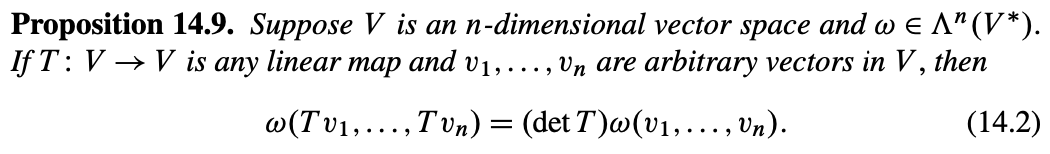
\includegraphics[scale=0.5]{prop14.9.png}}
así que
\begin{align*}
dV(\widetilde{E}_1,...,\widetilde{E}_n)&=\epsilon^1\wedge...\wedge\epsilon^n(\widetilde{E}_1,...,\widetilde{E}_n)\\
&=(\det{A^j_i})\epsilon^1\wedge...\wedge\epsilon^n(E_1,...,E_n)\\
&=\det{A^j_i}
\end{align*}
Ahora como los dos marcos son ortonormales, la matriz $(A^j_i)$ es una transformación lineal que preserva la métrica y fija el origen, de tal forma que es una matriz ortogonal en el grupo $O(n)$. Y como además las dos bases son orientadas, podemos suponer que $\det{A^j_i}=1$.\par
Ahora veamos la unicidad de $dV$. Tomemos $dV$ de acuerdo a la definición que hemos dado y supongamos que $\alpha$ es otra forma diferenciable que satisface (2). Notemos que $\bigwedge^n(M)$ está generada por $dV$, de forma que debe existir $f$ suave tal que $dV=f\alpha$. Basta mostrar que $f=1$. Y sí, porque
$$1=dV(E_1,...,E_n)=\alpha(E_1,...,E_n)$$
Por último comprobemos la equivalencia de (3). Como en los incisos anteriores, partimos de que existen funciones suaves $f$ y $A^i_j$ tales que
$$dV=fdx^1\wedge...\wedge dx^n \qquad\qquad \text{y} \qquad \qquad\partial x_i=A^j_iE_j$$
Entonces:
\begin{align*}
f&=fdx^1\wedge...\wedge dx^n(\partial x_1,...,\partial x_n)\\
&=dV(\partial x_1,...,\partial x_n)\\
&=dV(A^j_1E_j,...,A^j_nE_n)\\
&=\det{A^j_i}dV(E_1,...,E_n)\\
&=\det{A^j_i}
\end{align*}
Por otro lado, tenemos:
\begin{align*}g_{ij}&=\langle \partial x_i,\partial x_j\rangle=\langle A^k_i E_k,A^\ell_jE_\ell\rangle\\
&=A^k_iA^\ell_j\langle E_k,E_\ell\rangle=A^k_iA^\ell_j\delta_{k\ell}=\sum_kA^k_iA^k_j
\end{align*}
luego este número es la entrada $(i,j)$ de la matriz $A^TA$ y así
$$\det{g_{ij}}=\det{A^TA}=\det{A^T}\det{A}=(\det{A})^2$$
De esta forma, $f=\pm\sqrt{\det{A}}$. Como los dos marcos son orientados, por definición el determinante de la matriz $(A^i_j)$ debe ser positivo, y como este determinante es justamente $f$, tomamos el signo positivo y hemos terminado.\par
Observación: falta comprobar que (3) implica (2).\newpage

\section*{Inmersión isométrica del toro plano en $\mathbb R^2$}
\textbf{Dé una inmersión isométrica del toro plano, $\mathbb{T}^n$ a $\mathbb{R}^{2n}$.}\par
(Creo que no está del todo bien) Para dar una definición correcta de $\mathbb{T}^n$, consideremos la función 
\begin{align*}
\varphi:\mathbb{R}^n&\longrightarrow\mathbb{R}^{2n}\\(\theta_1,...,\theta_n)&\mapsto(\cos{\theta_1},\sin{\theta_1},...,\cos{\theta_n},\sin{\theta_n})
\end{align*}
y veamos que es una inmersión isométrica cuya imagen es $\mathbb{T}^n=\underbrace{\mathbb{S}^1\times...\times\mathbb{S}^1}_{n\text{ veces}}$.\par
En primer lugar,
\begin{equation*}
    d_p\varphi =
\begin{pmatrix}
-\sin{\theta_1}& 0&\cdots&0\\
\cos{\theta_1}&0&\cdots&0\\
\vdots&\vdots&\ddots&\vdots\\
0&0&\cdots&-\sin{\theta_n}\\
0&0&\cdots&\cos{\theta_n}\\
\end{pmatrix}
\end{equation*}
es de rango máximo, por lo que es inyectiva en cualquier punto.\par
Para ver que se trata de una isometría, basta notar que
$$\langle d_p\varphi e_i,d_p\varphi e_j\rangle=\langle (0,\cdots, -\sin{\theta_i},\cos{\theta_i},\cdots,0),(0,\cdots,-\sin{\theta_j},\cos{\theta_j},\cdots,0)\rangle=\delta_{ij}=\langle e_i,e_j\rangle$$
Una inmersión isométrica de $\mathbb{T}^n$ a $\mathbb{R}^{2n}$ es la identidad restringida a la imagen de $\varphi$.

\newpage
\section*{Transporte paralelo en el cono}
\textbf{Considere la esfera $S^2\subset\mathbb{R}^2$. Sea $\gamma$ un paralelo de latitud $\psi$. (Por lo que, si $(\theta,\varphi)\in[0,2\pi]\times[0,\pi]$ son coordenadas esféricas sobre $S^2$, entonces $\psi=\pi/2-\varphi$). Sea $\mathbf{V}_0$ un vector tangente a $S^2$ en algún punto de $\gamma$, y sea $\alpha_0$ el ángulo que forma $\mathbf{V}_0$ con $\gamma$. Deduzca una expresión para $\alpha$, el ángulo que forma el transporte paralelo de $\mathbf{V}_0$ a lo largo de $\gamma$, en términos de la latitud $\psi$ y la longitud del recorrido sobre $\gamma$. En particular, encuentre una expresión para $\alpha$ cuando el recorrido es una vuelta completa sobre $\gamma$.}\par

\textit{Sugerencia: considere el cono tangente a $S^2$ a lo largo de $\gamma$. Demuestre que el transporte paralelo de $\mathbf{V}_0$ a lo largo de $\gamma$ no depende de si se toma relativo a $S^2$ o al cono.}\par
\textbf{Una observación de Dani unos meses después… ¿Qué no podemos simplemente, como Do Carmo, suponer que nuestro paralelo $\gamma$ está parametrizado por longitud de arco y así la relación entre $s$ y $\theta$ es trivial? (son iguales) Al final, para calcular $\alpha$ tras una vuelta completa, volvemos a obtener $2\pi\sin\psi+\alpha_0$.}\par
(Consultar do Carmo, Geometría diferencial de curvas y superficies). Supongamos por ahora que la sugerencia es cierta y que hay una isometría local natural entre el cono menos una generatriz y una región abierta de $\mathbb{R}^2$. 
\begin{center}
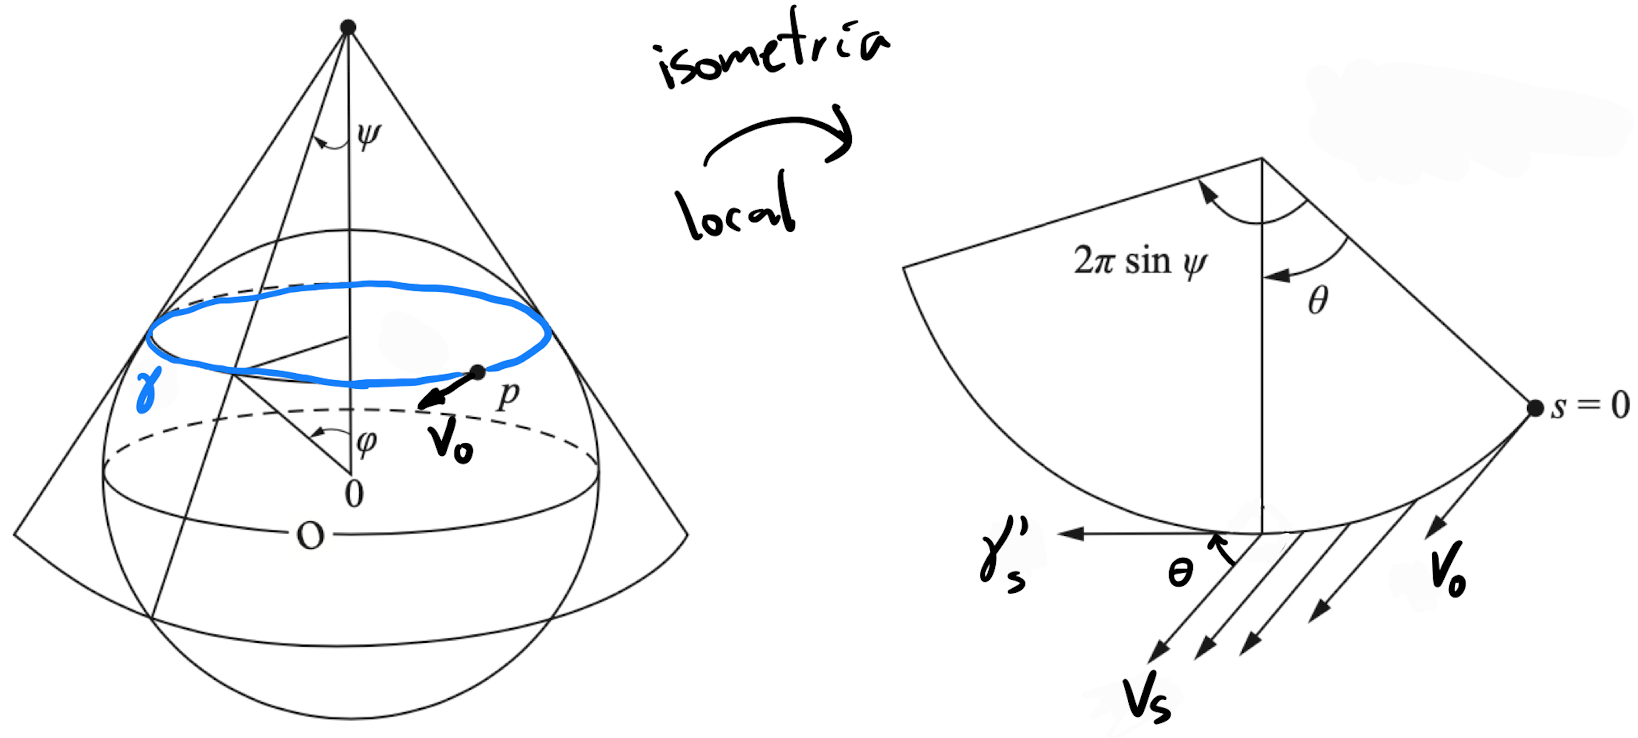
\includegraphics[scale=0.39]{img1.png}
\end{center}
Comenzaremos por observar que, en el caso en el que $\mathbf{V}_0$ fuera el vector velocidad de una parametrización por longitud de arco de $\gamma$, el ángulo orientado entre el transporte paralelo de $\mathbf{V}_0$ y $\gamma'$ tras un desplazamiento de ángulo central $\theta$ sería exactamente de $\theta$. Esto se debe a las dos suposiciones del párrafo anterior y a que el transporte paralelo en el plano es trivial.\par
Acercándonos a nuestro problema, si $\mathbf{V}_0$ fuera cualquier otro vector cuyo ángulo con el vector $\gamma'_0$ fuera de $\alpha_0$, no queda más remedio que el ángulo orientado entre el transporte paralelo de $\mathbf{V}_0$ y $\gamma'$ después de un desplazamiento de ángulo central $\theta$ sea de $\alpha_0+\theta=\alpha$.
\begin{center}
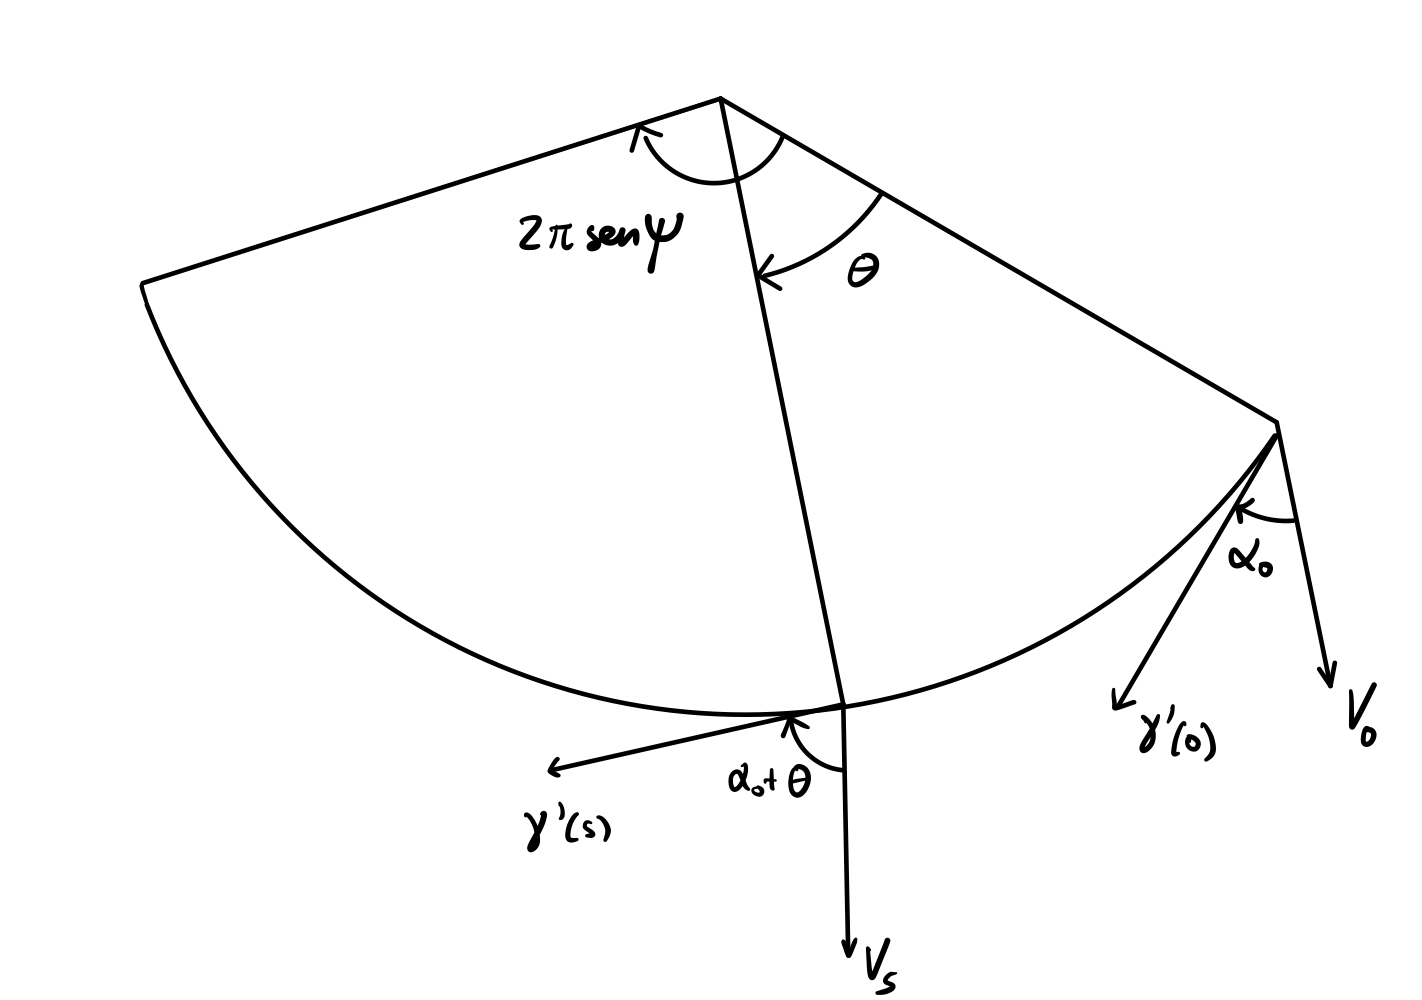
\includegraphics[scale=0.13]{img2.png}
\end{center}
Para dar una descripción de $\alpha$ en términos de la latitud $\psi$ y la longitud del recorrido sobre $\gamma$ basta dar la relación entre el ángulo central del recorrido $\theta$ y la longitud del recorrido $s$. Esto depende del tamaño del paralelo, que está determinado por $\psi$.\par
Un desplazamiento de longitud $s$ a lo largo de un círculo unitario cssorresponde con un ángulo central $\theta=s$. Si el círculo es de radio $r$, un desplazamiento de longitud $s$ corresponde con un ángulo central $\theta=s/r$.
\begin{center}
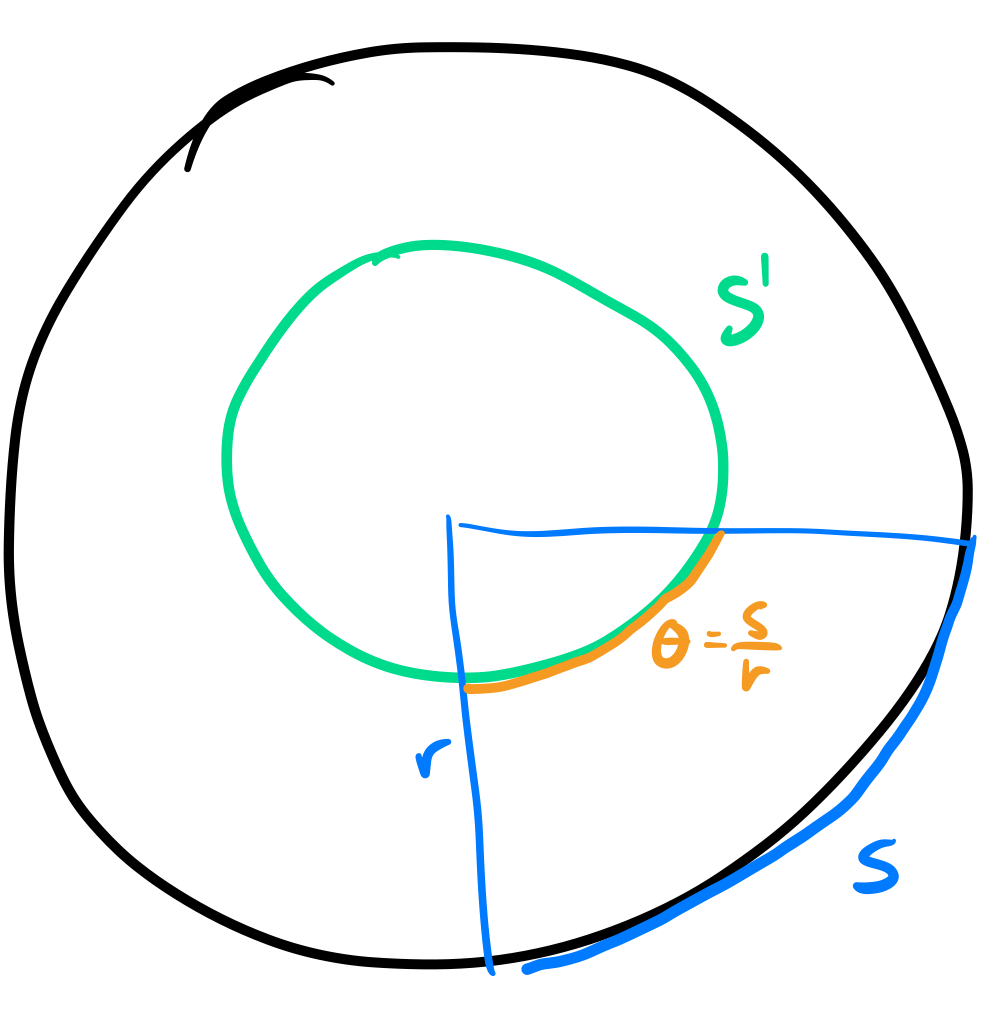
\includegraphics[scale=0.1]{img3.png}
\end{center}
Por último, el radio del círculo $r$ está dado por el dibujo y la ecuación de Mara:
\begin{center}
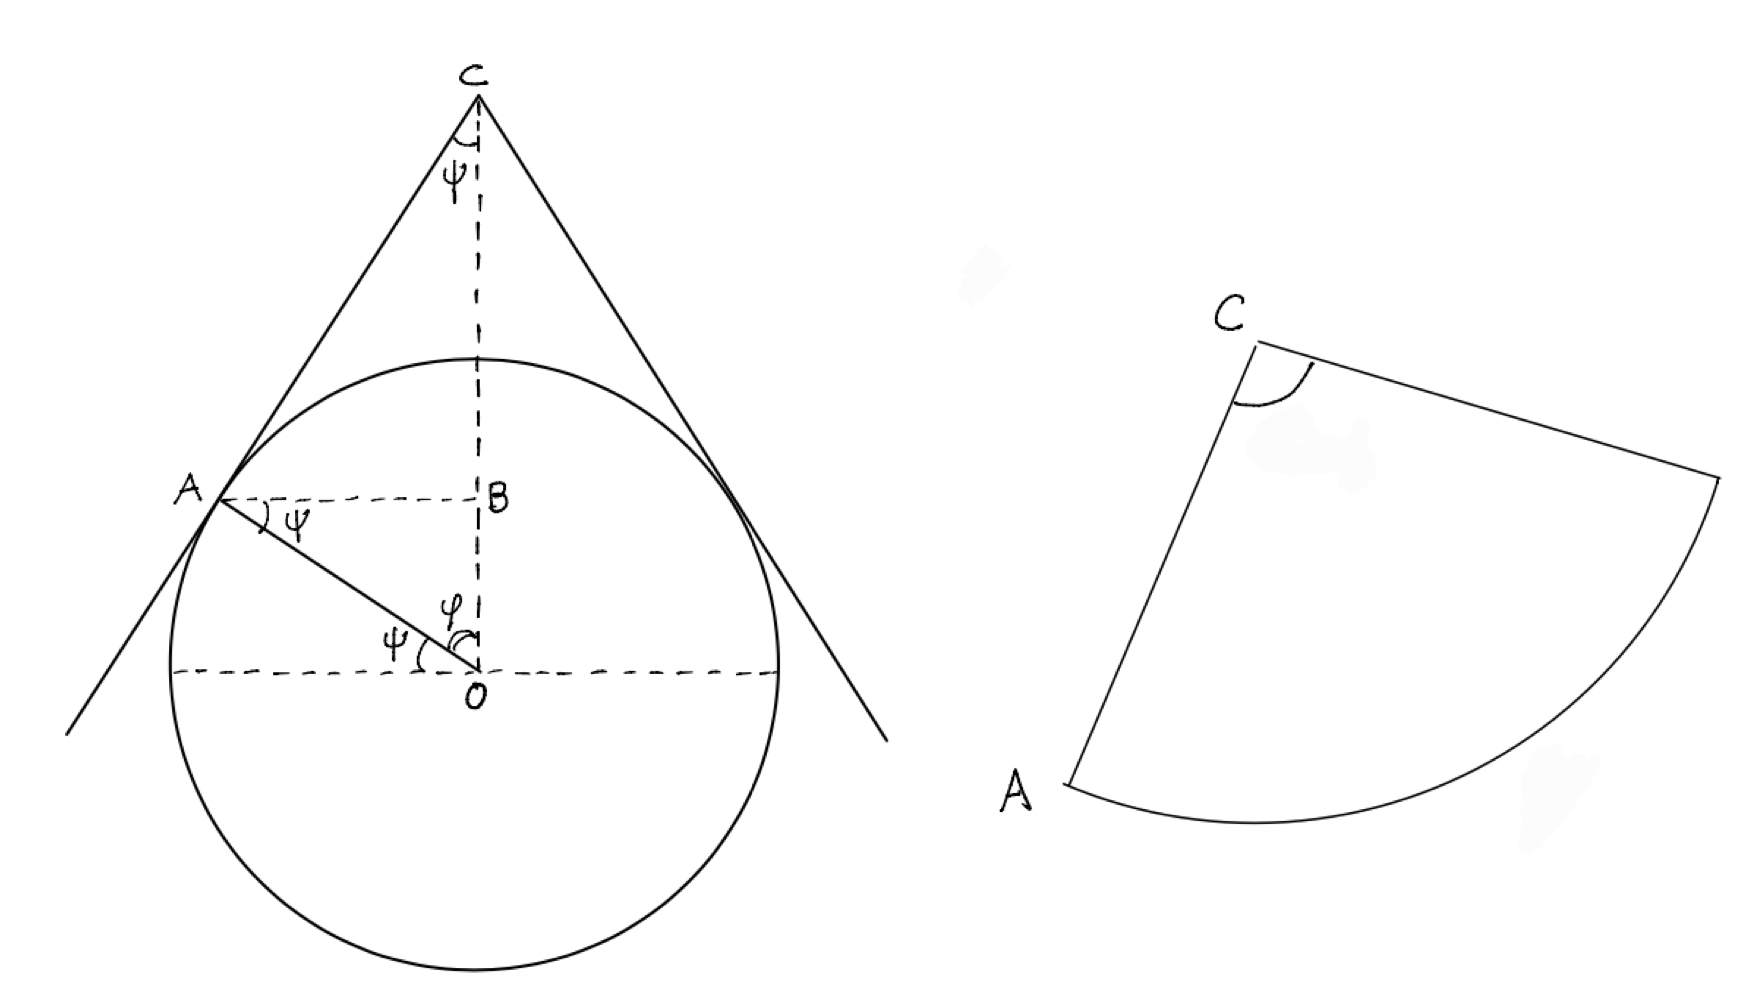
\includegraphics[scale=0.2]{img4.png}
\end{center}
$$r=CA=\sqrt{(OC)^2-1}=\sqrt{\csc^2\psi-1}=\cot\psi$$
Así que
$$\theta=\frac{s}{\cot\psi}=s\tan\psi$$
Y por fin
$$\alpha=\alpha_0+s\tan\psi$$
En el caso de la vuelta completa sobre $\gamma$, $$s=2\pi AB=2\pi\frac{\text{sen }\psi}{\tan\psi}$$ y entonces $\alpha=\alpha_0+2\pi\text{sen }\psi$.\par
Ahora volvamos para confirmar que el transporte paralelo es el mismo para cualquier superficie tangente a una curva. Para hacer una prueba general, tomemos $S$ y $S'$ dos superficies que contienen una curva $\gamma$ tales que $T_pS=T_pS'$ para cualquier $p\in\gamma$. Veamos que la derivada covariante a lo largo de $\gamma$ coincide en ambas superficies.\par
En el contexto de superficies regulares encajadas en $\mathbb{R}^3$, la derivada covariante de cualquier campo vectorial $\mathbf{V}$ definido sobre $\gamma$ es la proyección sobre el plano tangente de la derivada usual del campo visto como función de $\mathbb{R}^2$ en $\mathbb{R}^3$, y al coincidir los planos tangentes se sigue inmediante que la derivada covariante coincide.\par
Para una demostración usando la definición de los símbolos de Christoffel, basta tomar dos parametrizaciones locales de $S$ y $S'$ que coincidan en los vectores básicos del plano tangente a lo largo de $\gamma$ para obtener una igualdad en los símbolos de Christoffel de cada derivada covariante y también mismas funciones componentes del campo $\mathbf{V}$ a lo largo de $\gamma$, de lo que se sigue que las derivadas covariantes coinciden a lo largo de $\gamma$.\par
Usando cualquiera de estos argumentos, concluimos que el transporte paralelo de un vector $\mathbf{V}_0\in\gamma$ coincide para ambas superficies porque el transporte paralelo es único (Teo. de existencia y unicidad).\par
Por último, la isometría local entre el cono tangente al paralelo menos una generatriz y la región de $\mathbb{R}^2$ delimitada en coordenadas polares por
$$0<\rho,\quad \quad\quad 0<\theta<2\pi\text{sen }\psi$$
se puede dar usando una aplicación que preserva la primera forma fundamental del cono y la del plano de acuerdo una parametrización con coordenadas polares. Precisamente por preservar la primera forma fundamental, dos superficies localmente isométricas tienen el mismo transporte paralelo, y hemos terminado.
\newpage

\section*{Integral de la curvatura escalar en la esfera}
\textbf{Pruebe que la curvatura escalar en un punto $p$ de una variedad Riemanniana $n$-dimensional $M$ está dada por}
$$K(p)=\frac{1}{\omega_{n-1}}\int_{S^{n-1}}\text{Ric}_p(x)dS^{n-1}$$
\textbf{de acuerdo a las definiciones}
$$K(p):=\frac{1}{n}\sum_i\text{Ric}_p(e_i)$$
\textbf{y}
$$\text{Ric}_p(e_i):=\frac{1}{n-1}\sum_{i\neq j}\langle R(e_i,e_j)e_i,e_j\rangle$$
\textbf{para una base ortonormal $\{e_i\}$ de $T_pM$.}\par
Como la función escalar $\text{Ric}_p$ es una forma bilineal simétrica, sabemos que existen $\lambda_i$ tales que si un vector tangente $x\in T_pM$ está dado por $x=\sum_ix_ie_i$, entonces
$$\text{Ric}_p(x)=\sum_i \lambda_ix_i^2.$$
Como la integral está dada en la esfera unitaria, tendremos que $|x|=1$, y entonces el vector en $\mathbb{R}^n$ definido por $\nu=(x_1,...,x_n)$ también es unitario. Definamos también el vector $V=(\lambda_1x_1,...,\lambda_nx_n)$. Con esto, nuestra integral se puede ver como
$$\frac{1}{\omega_{n-1}}\int_{S^{n-1}}\text{Ric}_p(x)dS^{n-1}=\frac{1}{\omega_{n-1}}\int_{S^{n-1}}\langle V,\nu\rangle dS^{n-1}$$
Aplicando teorema de la divergencia vía Stokes y el hecho de que $\text{vol }B^n/\omega_{n-1}=1/n$ obtenemos:
\begin{align*}
    \frac{1}{\omega_{n-1}}\int_{S^{n-1}}\langle V,\nu\rangle dS^{n-1}&=\frac{1}{\omega_{n-1}}\int_{B^n}\text{div }VdB^n\\
    &=\frac{1}{n}\text{div }V\\
    &=\frac{\sum\lambda_i}{n}\\
    &=\frac{\sum\text{Ric}_p(e_i)}{n}\\
    &=K(p)
\end{align*}
Observación: las dos primeras igualdades en la expresión anterior requieren justificación.
\newpage
\section*{Pullback de una forma diferencial}

Sean $F:M\longrightarrow N$ una función suave y  $\omega$ una $k$-forma diferencial en $N$. El \textbf{pullback} de $\omega$ es una $k$-forma en $M$ dada por  
\begin{equation*}
(F^*\omega)_p(v_1,...,v_k)=\omega_{F(p)}(dF_pv_1,...,dF_{p}v_k)
\end{equation*}
para $p\in M$ y $v_1,...,v_k$ vectores en $T_pM$.

Eventualmente se definirá la integral de una forma (que puede medir un volumen) en una variedad usando el pullback de una carta coordenada:
\begin{equation*}
    \int_U\omega=\int_{\phi(U)}(\phi^{-1})^*\omega
\end{equation*}
llevando así la integral a $\mathbf{R}^n$. \par
    \par\textbf{Lema 14.16}. Para $F:M\longrightarrow N$ suave,
    \begin{enumerate}[label=(\alph*)]
        \item $F^*:\Omega^k(N)\longrightarrow\Omega^k(M)$ es lineal sobre $\mathbf{R}$
        \item $F^*(\omega\wedge\eta)=F^*\omega\wedge F^*\eta$
        \item En cualquier carta coordenada,
        \begin{equation*}
            F^*\left(\sum_{I}^{\big'}\omega_Idy^{i_1}\wedge ...\wedge dy^{i_k}\right)=\sum_I^{}^{\big'} (\omega_I\circ F) d(y^{i_1}\circ F)\wedge ...\wedge  d(y^{i_k}\circ F)
        \end{equation*}
    \end{enumerate}

\par \emph{Demostración.}
\begin{enumerate}[label=(\alph*)]
    \item Para $a\in \mathbf{R}$ y dos $k$-formas en $N$,
    \begin{align*}
        (F^*(a\omega+\eta))_p(v_1,...,v_k) &=(a\omega+\eta)_{F(p)}(dF_{p}v_1,...,dF_{p}v_k)\\
        &=a\omega_{F(p)}(dF_{p}v_1,...,dF_{p}v_k)+\eta_{F(p)}(dF_{p}v_1,...,dF_{p}v_k)\\
        &=a(F^*\omega)_p(v_1,...,v_k)+(F^*\eta)_p(v_1,...,v_k)
    \end{align*}
    \item
    \begin{align*}
        (F^*(\omega\wedge \eta))_p(v_1,...,v_{k+l})&=(\omega\wedge \eta)_{F(p)}(dF_{p}v_1,...,dF_{p}v_{k+l})\\
        &=(\omega_{F(p)}\wedge \eta_{F(P)})(dF_{p}v_1,...,dF_{p}v_{k+l})\\
        &=\frac{(k+l)!}{k!l!}\text{Alt}(\omega_{F(p)}\otimes\eta_{F(p)})(dF_{p}v_1,...,dF_{p}v_{k+l})\\
        &=\frac{1}{k!l!}\sum \text{sgn}(\sigma)\omega_{F(p)}(dF_{p}v_{\sigma(1)},...,dF_{p}v_{\sigma(k)})\\ &\quad\quad\quad\quad\quad\quad\quad\quad\quad\quad\quad\quad\quad\quad\quad
        \cdot\eta_{F(p)}(dF_{p}v_{\sigma(k+1)},...,dF_{p}v_{\sigma(l)})\\
        &=\frac{1}{k!l!}\sum \text{sgn}(\sigma)F^*\omega(v_{\sigma(1)},...,v_{\sigma(k)})F^*\eta(v_{\sigma(k+1)},...,v_{\sigma(k+l)})\\
        &= \frac{(k+l)!}{k!l!}\text{Alt}((F^*\omega)_p\otimes(F^*\eta)_p)(v_1,...,v_{k+l})\\
        &= (F^*\omega)_p\wedge (F^*\eta)_p(v_1,...,v_{k+l})
    \end{align*}

    \item En clase vimos un caso muy sencillo pensando en $N=\mathbf{R}^2$ con coordenadas $(y^1,y^2)$. Mostramos que el pullback de una 2-forma $\omega=\omega_{12}dy^1\wedge dy^2$ es:
    \begin{align*}
        F^*(\omega_{12}dy^1\wedge dy^2)_p(v_1,v_2)&=(\omega_{12}dy^1\wedge dy^2)_{F(p)}(dF_{p}(v_1),dF_{p}(v_2))\\
        &=\omega_{12}(F(p))\frac{1}{1!1!}\sum\text{sgn}(\sigma)dy^1_{F(p)}(dF_p(v_{\sigma(1)})dy^2_{F(p)}(dF_p(v_{\sigma(2)})\\
        &=(\omega_{12}\circ F)(p)\sum\text{sgn}(\sigma)d(y^1\circ F)_p(v_{\sigma(1)})d(y^2\circ F)_p(v_{\sigma(2)})\\
        &=(\omega_{12}\circ F)(p)(d(y^1\circ F)_p\wedge d(y^2\circ F)_p)(v_1,v_2)\\
        &=(\omega_{12}\circ F)(p)(d(y^1\circ F)\wedge d(y^2\circ F))_p(v_1,v_2)\\
    \end{align*}
    Comentamos que esta prueba se puede tomar como el caso base para una inducción sobre $k$ en una variedad $N$ de dimensión $n$. (En la prueba nunca usamos que la dimensión de $N$ fuera 2.)
\end{enumerate}
\newpage

\section*{Ley de transformación para los coeficientes de una conexión}
\textbf{Sean $M$ una variedad suave con o sin frontera y $\nabla$ una conexión en $TM$. Tomemos dos marcos locales $(E_i)$ y $(\widetilde{E}_j)$ de $TM$ en algún abierto $U\subseteq M$. Supongamos que se tiene la relación }
\begin{equation}
    \widetilde{E}_i=A_i^jE_j
\end{equation}\textbf{para alguna matriz de funciones $A_i^j$. Si los coeficientes de Christoffel de $\nabla$ respecto a $(E_i)$ son $\Gamma_{ij}^k$ y respecto a  $(\widetilde{E}_j)$ son $\widetilde\Gamma_{ij}^{k}$, entonces $$\widetilde{\Gamma}_{ij}^k=\left(A^{-1}\right)_p^kA_i^qA_j^r\Gamma_{qr}^p+\left(A^{-1}\right)_p^kA_i^qE_q(A_j^p)$$}

\textit{Demostración}\par Sabemos que:
$$\nabla_{\widetilde{E}_i}\widetilde{E}_j=\widetilde{\Gamma}_{ij}^k\widetilde{E}_k$$

Y sustituyendo con (1):
    $$\nabla_{A_i^qE_q}(A_j^pE_p)=\widetilde{\Gamma}_{ij}^kA_k^rE_r$$
Ahora volteemos la identidad anterior y usemos las propiedades de linealidad y Leibniz de $\nabla$:
\begin{align*}
    \widetilde{\Gamma}_{ij}^kA_k^rE_r&=A_i^q\nabla_{E_q}(A_j^pE_p)\\
    &=A_i^q\left(E_q(A_j^p)E_p+A_j^p\nabla_{E_q}E_p\right)\\
    &=A_i^q\left(E_q(A_j^p)E_p+A_j^p\Gamma_{qp}^rE_r\right)\\
    &=A_i^qE_q(A_j^p)E_p+A_i^qA_j^p\Gamma_{qp}^rE_r
\end{align*}
Notemos que en él último sumando de la última expresión los índices $p$ y $r$ son mudos. Comparando con el resultado al que queremos llegar, conviene intercambiarlos. De una vez también vamos a intercambiar la $r$ por la $p$ en el lado izquierdo de la ecuación. Obtenemos:
\begin{align*}
\widetilde{\Gamma}_{ij}^kA_k^pE_p&=A_i^qE_q(A_j^p)E_p+A_i^qA_j^r\Gamma_{qr}^pE_p
\end{align*}
Podemos quitar el campo $E_p$ para obtener que dada una $p$,
\begin{align*}
 \widetilde{\Gamma}_{ij}^kA_k^p&=A_i^qE_q(A_j^p)+A_i^qA_j^r\Gamma_{qr}^p\\
%\end{align*}
 \iff (A^{-1})_p^kA_k^p\widetilde{\Gamma}_{ij}^k&=(A^{-1})_p^kA_i^qE_q(A_j^p)+(A^{-1})_p^kA_i^qA_j^r\Gamma_{qr}^p\\
 \iff\widetilde{\Gamma}_{ij}^k
 &=(A^{-1})_p^kA_i^qE_q(A_j^p)+(A^{-1})_p^kA_i^qA_j^r\Gamma_{qr}^p
\end{align*}
Donde el último paso se puede pensar como un producto de matrices.
%Para el último paso tomemos un índice fijo $s$ y multipliquemos por la función $(A^{-1})_p^s$:
%\begin{align*}
% (A^{-1})_p^sA_k^p\widetilde{\Gamma}_{ij}^k&=(A^{-1})_p^sA_i^qE_q(A_j^p)+(A^{-1})_p^sA_i^qA_j^r\Gamma_{qr}^p\\
%\end{align*}
\newpage

\section*{Pullback de una conexión}

\textbf{Sean $M$ y $\widetilde{M}$ variedades suaves con o sin frontera. Supongamos que $\widetilde{\nabla}$ es una conexión en $T\widetilde{M}$ y $\varphi:M\longrightarrow\widetilde{M}$ es un difeomorfismo. Entonces, el mapeo}
$$\varphi^*\widetilde{\nabla}:\mathfrak{X}(M)\times\mathfrak{X}(M)\longrightarrow\mathfrak{X}(M)$$
\textbf{dado por}
$$(\varphi^*\widetilde{\nabla})_XY=(\varphi^{-1})_*\widetilde{\nabla}_{\varphi_*X}\varphi_*Y$$
\textbf{es una conexión en $TM$.}\par
\textit{Esta proposición sirve para demostrar la naturalidad de la conexión de Levi-Civita: si $\varphi$ fuera una isometría de variedades Riemannianas, el pullback de la conexión de Levi-Civita de $\widetilde{M}$ es la conexión de Levi-Civita de $M$.}\par
Vamos a la demostración. Hay que ver que $\varphi^*\widetilde{\nabla}$ es $\mathbb{R}$-lineal en el segundo argumento, $\mathcal{C}^\infty$-lineal en el primer argumento y Leibniz en el segundo argumento.\par
\begin{enumerate}
    \item
    \begin{align*}        (\varphi^*\widetilde{\nabla})_X(aY_1+Y_2)&=(\varphi^{-1})_*\widetilde{\nabla}_{\varphi_*X}\varphi_*(aY_1+Y_2)\\
     &=(\varphi^{-1})_*\widetilde{\nabla}_{\varphi_*X}(a\varphi_*Y_1+\varphi_*Y_2)\\
     &=(\varphi^{-1})_*(a\widetilde{\nabla}_{\varphi_*X}\varphi_*Y_1+\widetilde{\nabla}_{\varphi_*X}\varphi_*Y_2)\\
     &=a(\varphi^{-1})_*\widetilde{\nabla}_{\varphi_*X}\varphi_*Y_1+(\varphi^{-1})_*\widetilde{\nabla}_{\varphi_*X}\varphi_*Y_2\\
     &=a(\varphi^*\widetilde{\nabla})_XY_1+(\varphi^*\widetilde{\nabla})_XY_2
    \end{align*}

    \item 
    \begin{align*}        (\varphi^*\widetilde{\nabla})_{(fX_1+X_2)}Y&=(\varphi^{-1})_*\widetilde{\nabla}_{\varphi_*(fX_1+X_2)}\varphi_*Y\\
     &=(\varphi^{-1})_*\widetilde{\nabla}_{\varphi_*fX_1+\varphi_*X_2}Y\\
     &=(\varphi^{-1})_*\widetilde{\nabla}_{(f\circ\varphi^{-1})\varphi_*X_1+\varphi_*X_2}Y
    \end{align*}
    Definamos $\tilde{f}=f\circ\varphi^{-1}$ para obtener
    \begin{align*}        (\varphi^*\widetilde{\nabla})_{(fX_1+X_2)}\varphi_*Y&=(\varphi^{-1})_*\widetilde{\nabla}_{\tilde{f}\varphi_*X_1+\varphi_*X_2}\varphi_*Y\\
    &=(\varphi^{-1})_*(\tilde{f}\widetilde{\nabla}_{\varphi_*X_1}\varphi_*Y+\widetilde{\nabla}_{\varphi_*X_2}\varphi_*Y)\\
    &=(\varphi^{-1})_*(\tilde{f}\widetilde{\nabla}_{\varphi_*X_1}\varphi_*Y)+(\varphi^{-1})_*\widetilde{\nabla}_{\varphi_*X_2}\varphi_*Y\\
    &=\tilde{f}\circ\varphi^{-1}(\varphi^{-1})_*\widetilde{\nabla}_{\varphi_*X_1}\varphi_*Y+(\varphi^{-1})_*\widetilde{\nabla}_{\varphi_*X_2}\varphi_*Y\\
    &=f(\varphi^{-1})_*\widetilde{\nabla}_{\varphi_*X_1}\varphi_*Y+(\varphi^{-1})_*\widetilde{\nabla}_{\varphi_*X_2}\varphi_*Y\\
    &=f(\varphi^*\widetilde{\nabla})_{X_1}\varphi_*Y+(\varphi^*\widetilde{\nabla})_{X_2}\varphi_*Y
    \end{align*}
\newpage
    \item Usando la misma notación para $\tilde{f}$,
    \begin{align*}        (\varphi^*\widetilde{\nabla})_{X}(fY)&=(\varphi^{-1})_*\widetilde{\nabla}_{\varphi_*X}\varphi_*(fY)\\
     &=(\varphi^{-1})_*\widetilde{\nabla}_{\varphi_*X}\tilde{f}\varphi_*\varphi_*Y\\
     &=(\varphi^{-1})_*\left( \varphi_*X\tilde{f}\varphi_*Y+\tilde{f}\widetilde{\widetilde{\nabla}_}{\varphi_*X}\varphi_*Y\right)\\
     &=(\varphi^{-1})_*\varphi_*X\tilde{f}\varphi_*Y+(\varphi^{-1})_*(\tilde{f}\widetilde{\nabla}_{\varphi_*X}\varphi_*Y)\\
     &=(\varphi_*X\tilde{f}\circ\varphi^{-1})(\varphi^{-1})_*\varphi_*Y+(\tilde{f}\circ\varphi^{-1})(\varphi^{-1})_*\widetilde{\nabla}_{\varphi_*X}\varphi_*Y\\
     &=Xf(\varphi^{-1})_*\varphi_*Y+f(\varphi^{-1})_*\widetilde{\nabla}_{\varphi_*X}\varphi_*Y\\
     &=XfY+f(\varphi^*\widetilde{\nabla})_{X}Y
    \end{align*}
*Faltó aclarar la igualdad del primer sumando en el último paso*
\end{enumerate}
\newpage

\section*{Campos vectoriales y flujos}
\textbf{(Problemas de Flujos \#4). Dé un ejemplo de campos vectoriales $X,Y$ y $W$ en $\mathbb{R}^2$ tales que $X=Y=\frac{\partial}{\partial x} $ a lo largo del eje $x$ pero que $\mathcal{L}_XW\neq\mathcal{L}_YW$}.\par
Consideremos los campos que hacen esto algebraicamente más sencillo:
$$X=\frac{\partial}{\partial x}$$
$$Y=\frac{\partial}{\partial x}+y\frac{\partial}{\partial y}$$
(Así $Y$ se vuelve $\frac{\partial}{\partial x}$ en el eje $x$.)\par
Veamos si funciona:
\begin{align*}
    \mathcal{L}_XW_p(f)&=[X,W]_p(f)\\
    &=X_pW(f)-W_pX(f)\\
    &=\frac{\partial W(f)}{\partial x}\bigg\rvert_p-W_p\left(\frac{\partial f}{\partial x}\right)
\end{align*}
Mientras que
\begin{align*}
    \mathcal{L}_YW_p(f)&=[Y,W]_p(f)\\
    &=Y_pW(f)-W_pY(f)\\
    &=\left(\frac{\partial}{\partial x}+y\frac{\partial}{\partial y}\right)_pW(f)-W_p\left(\frac{\partial }{\partial x}+y\frac{\partial }{\partial y}\right)f\\
    &=\frac{\partial W(f)}{\partial x}\bigg\rvert_p+y\frac{\partial W(f)}{\partial y}\bigg\rvert_p-W_p\left(\frac{\partial f}{\partial x}\right)-W_p\left(y\frac{\partial f}{\partial y}\right)\\
    &=\mathcal{L}_XW_p(f)+y\frac{\partial W(f)}{\partial y}\bigg\rvert_p-W_p\left(\frac{\partial f}{\partial x}\right)
\end{align*}
Así que, por ejemplo,
$$W=\frac{\partial}{\partial x}$$
implicaría que
\begin{align*}
    y\frac{\partial W(f)}{\partial y}\bigg\rvert_p-W_p\left(\frac{\partial f}{\partial x}\right)&=y\frac{\partial}{\partial y}\bigg\rvert_p\left(\frac{\partial f}{\partial x}\right)-\frac{\partial}{\partial x}\bigg\rvert_p\left(\frac{\partial f}{\partial x}\right),
\end{align*}
que no se hace cero en el origen para todas las funciones continuas y por lo tanto $\mathcal{L}_XW_{(0,0)}-\mathcal{L}_YW_{(0,0)}\neq 0$.
\newpage

\section{Flujos y homotopía}
\textbf{(Flujos \#3) Supongamos que $M$ es una variedad suave y compacta que admite un campo vectorial que no se anula en ninguna parte. Demuestre que existe un mapeo suave $F:M\longrightarrow M$ que es homotópico a la identidad y no tiene puntos fijos.}\\ \par
    
Tomemos un campo vectorial $X$ en $M$ que no se anule en ninguna parte, de forma que existan coordenadas locales $(x^1,...,x^n)$ tales que  $X=\frac{\partial }{\partial x^1}$ en una vecindad de cualquier punto. En este caso, una curva integral $\theta(t,p)$ de $X$ tiene coordenadas $(p^1+t,0,...,0)$ cerca de $p$. Una curva de este estilo puede tomar valores de $t$ siempre que no se salga del abierto donde tenemos esas coordenadas, así que nuestra variable se mueve en un dominio acotado, digamos $0\leq t\leq t_p$.\par
Hemos construido una cubierta abierta $\{U_p\}_{p\in M}$ de nuestra variedad, que es compacta, así que hay una subcubierta finita $\{U_i\}_{i=1}^{k}$. A cada uno de estos abiertos corresponde un valor máximo al que puede llegar el parámetro de las curvas integrales, digamos $t_i$.\par
Tomemos $T=\min t_i$ y la función $F:M\longrightarrow M$ que, digamos, ``avanza T unidades de tiempo" a lo largo de las curvas integrales de $X$. Dicho de otra forma, $F(p)=\theta(p,T)$.\par
Ya tenemos una función, sólo queda probar es homotópica a la identidad y que no tiene puntos fijos. Comencemos con lo segundo.\par
Cualquier punto $p$ de la variedad está contenido en uno de los $k$ abiertos de la subcubierta finita, donde la curva intgral que pasa por $p$ tiene coordenadas $(p^1+t,0,...,0)$. No queda de otra que $p=\theta(p,0)\neq\theta(p,T)=F(p).$\par
Finalmente, una homotopía con la identidad es $H(s,p)=\theta(p,sT)$.

    \newpage

\section*{Mapeos multilineales}
\textbf{(Álgebra tensorial 1) Sea V un espacio vectorial de dimensión finita. Existe un isomorfismo natural (i.e. independiente de la base) entre $T^{(k+l,l)}$ y el espacio de todos los mapeos multilineales:}
$$T:\underbrace{V^*\times...\times V^*}_{k \text{ veces}}\times \underbrace{V \times ... \times V}_{\ell \text{ veces}}\longrightarrow V$$
Para un mapeo multilineal $T$ como arriba podemos definir $$\hat{T}(\omega_1,...,\omega_{k+1},v_1,...,v_\ell)=\omega_{k+1}(T(\omega_1,...,\omega_k,v_1,...,v_\ell)$$\par
La asociación $T\mapsto \hat{T}$ es el isomorfismo que buscamos. La linealidad se sigue trivialmente de la linealidad $T$ y de la forma diferencial $\omega_{k+1}$. Para ver que es inyectiva hay que invocar el resultado de que si todos los funcionales de un espacio vectorial (en este caso $\omega_{k+1}$, que podemos variar libremente) se hacen cero en el mismo vector (en este caso $T(\omega_1,...,\omega_k,v_1,...,v_\ell$)), entonces ese vector debe ser el cero. *Falta*
\newpage
\section*{Lema de Poincaré para conjuntos estrellados}
\textbf{(Álgebra tensorial 2) Si $U$ es un subconjunto estrellado de $\mathbb{R}^n$ o $\mathbb{H}^n$, entonces cualquier 1-forma cerrada definida en $U$ es exacta.}\par

Mostraremos que
$$d\int_{\gamma_x}\omega=\omega$$
donde $\gamma_x(t)=tx$ para $0\leq t\leq1$.\par
(El resultado es válido para conjuntos estrellados centrados en 0, cosa que podemos suponer sin pérdida de generalidad porque la traslación adecuada manda formas cerradas en cerradas, y exactas en exactas.)\par
Supongamos que $\omega=\sum_{i=1}^n\omega_idx^i$. Para encontrar la derivada exterior de la integral basta encontrar sus derivadas parciales.
\begin{align*}
    \frac{\partial}{\partial x^j}\int_{\gamma_x}\omega(x)&=\frac{\partial}{\partial x^j}\int_0^1\sum_{i=1}^n\omega_i(tx)x^idt\\
    &=\int_0^1\sum_{i=1}^n\frac{\partial}{\partial x^j}\omega_i(tx)x^idt\\
    &=\int_0^1\left(\sum_{i=1}^n\frac{\partial \omega_i}{\partial x^j}(tx)tx^i+\omega_j(tx)\right)dt\\
    &=\int_0^1\left(\sum_{i=1}^n\frac{\partial \omega_j}{\partial x^i}(tx)tx^i+\omega_j(tx)\right)dt\\
    &=\int_0^1\frac{d}{dt}t\omega_{j}(tx)dt\\
    &=\omega_j(x)
    \end{align*}
    Usando que como $\omega$ es cerrada, $$\frac{\partial \omega_i}{\partial x^j}=\frac{\partial \omega_j}{\partial x^i}$$
\newpage
\section*{Tensores: cambios de coordenadas}
\textbf{1}\\ \\
Veamos primero que si $i\neq j$, $A_j^i=0$.
Consideremos las bases
\begin{equation*}
\begin{split}
    & \xi=\{v_1,...,v_i,...,v_j,...,v_n\}\\
    & \eta=\{v_1,...,v_i,...,2v_j,...,v_n\}\\
\end{split}
\end{equation*}
del espacio $V$ de dimensión $n$. También tenemos sus correspondientes bases duales:
\begin{equation*}
\begin{split}
    & \xi^*=\{v_1^*,...,v_i^*,...,v_j^*,...,v_n^*\}\\
    & \eta^*=\{v_1^*,...,v_i^*,...,(2v_j)^*,...,v_n^*\}\\
\end{split}
\end{equation*}
Entonces, 
\begin{equation*}
\begin{split}
    A(v_i^*,v_j) = {}^\xi & A^i_j={}^\eta A^i_j = A(v_i^*,2v_j)= 2A(v_i^*,v_j)\\
    \iff & A(v_i^*,v_j)=0\\
    \iff & {}^\xi A^i_j=0
\end{split}
\end{equation*}
para cualquier base de $V$.\\
{\footnotesize\color{red}

Como observación, notemos que si $i=j$, la ecuación anterior se vuelve
\begin{equation*}
\begin{split}
    A(v_j^*,v_j) = {}^\xi & A^j_j={}^\eta A^j_j = A((2v_j)^*,2v_j)= 2A(\tfrac{1}{2}v_j^*,v_j)=A(v_j^*,v_j)\\
\end{split}
\end{equation*}
ya que $(2v_j)^*=\tfrac{1}{2}v_j^*$ por la construcción natural de la base dual.}\\ \\ \par
Ahora veamos que $A_i^i=A_j^j$. Tomemos las bases ordenadas
\begin{equation*}
\begin{split}
    & \xi=\{v_1,...,v_i,...,v_j,...,v_n\}\\
    & \eta=\{v_1,...,v_j,...,v_i,...,v_n\}\\
\end{split}
\end{equation*}
y sus bases duales $\xi^*$ y $\eta^*$. Entonces,
\begin{equation*}
\begin{split}
     {}^\xi A^i_i={}^\eta A^i_i &\iff A(v_i^*,v_i)=A(v_j^*,v_j)\\
    &\iff {}^\xi A^i_i={}^\xi A^j_j
\end{split}
\end{equation*}
Para cualquier base de $V$. Tomando $A^i_i=\lambda$ se obtiene el resultado.
\\ \\
\textbf{2 (a)}\\ \\
Sean $p\in\mathbb{R}^3$ y $q\in\mathbb{R}^2$. Entonces: \par
\begin{equation*}
    \begin{split}
        v\otimes w(p,q) & = v(p)w(q)\\
        & = \left(\sum_i v_idx^i\right)(p)\left(\sum_j w_jdy^j\right)(q)\\
        & = \sum_i v_idx^i(p)\sum_j w_jdy^j(q)\\
        & = \sum_{i,j}v_iw_jdx^i(p) dy^j(q)\\
        & = \sum_{i,j}v_iw_jdx^i\otimes dy^j(p,q)\\
        & = \left( \sum_{i,j}v_iw_jdx^i\otimes dy^j \right) (p,q)\\
    \end{split}
\end{equation*}
\\ \\
\textbf{2 (b)}\\

Tenemos que:

\begin{equation*}
    \begin{split}
        T_A(v) & = (av_1+bv_2+cv_3)dx^1\\
        & + (dv_1+ev_2+fv_3)dx^2\\
        & + (gv_1+hv_2+iv_3)dx^3\\
    \end{split}
\end{equation*}

Y que:

\begin{equation*}
    \begin{split}
        T_B(w) & = (pw_1+qw_2)dy^1\\
        & + (rw_1+sw_2)dy^2\\
    \end{split}
\end{equation*}
\newpage
Así que:

\begin{equation*}
    \begin{split}
        T_A(v)\otimes T_B(w) & = (av_1+bv_2+cv_3)(pw_1+qw_2)dx^1\otimes dy^1\\
        & + (dv_1+ev_2+fv_3)(pw_1+qw_2)dx^2\otimes dy^1\\
        & + (gv_1+hv_2+iv_3)(pw_1+qw_2)dx^3\otimes dy^1\\
        & + (av_1+bv_2+cv_3)(rw_1+sw_2)dx^1\otimes dy^2\\
        & + (dv_1+ev_2+fv_3)(rw_1+sw_2)dx^2\otimes dy^2\\
        & + (gv_1+hv_2+iv_3)(rw_1+sw_2)dx^3\otimes dy^2\\
        & = (apv_1w_1+bpv_2w_1+cpv_3w_1+aqv_1w_2+bqv_2w_2+cqv_3w_3)dx^1\otimes dy^1\\
        & + (dpv_1w_1+epv_2w_1+fpv_3w_1+dqv_1w_2+eqv_2w_2+fqv_3w_3)dx^2\otimes dy^1\\
        & + (gpv_1w_1+hpv_2w_1+ipv_3w_1+gqv_1w_2+hqv_2w_2+iqv_3w_3)dx^3\otimes dy^1\\
        & + (arv_1w_1+brv_2w_1+crv_3w_1+asv_1w_2+bsv_2w_2+csv_3w_3)dx^1\otimes dy^2\\
        & + (drv_1w_1+erv_2w_1+frv_3w_1+dsv_1w_2+esv_2w_2+fsv_3w_3)dx^2\otimes dy^2\\
        & + (grv_1w_1+hrv_2w_1+irv_3w_1+gsv_1w_2+hsv_2w_2+isv_3w_3)dx^3\otimes dy^2\\
    \end{split}
\end{equation*}

Así es que para la base ordenada 
\begin{equation*} dx^1\otimes dy^1,dx^2\otimes dy^1,dx^3\otimes dy^1,dx^1\otimes dy^2,dx^2\otimes dy^2,dx^3\otimes dy^2
\end{equation*}
tenemos que:\\
\begin{equation*}
    \begin{pmatrix}
    ap & bp & cp & aq & bq & cq \\
    dp & ep & fp & dq & eq & fq \\
    gp & hp & ip & gq & hq & iq \\
    ar & br & cr & as & bs & cs \\
    dr & er & fr & ds & es & fs \\
    gr & hr & ir & gs & hs & is \\
    \end{pmatrix}
    \begin{pmatrix}
    v_1w_1\\
    v_2w_1\\
    v_3w_1\\
    v_1w_2\\
    v_2w_2\\
    v_3w_2\\
    \end{pmatrix}
\end{equation*}
\\ es el vector de coordenadas de $(T_A\otimes T_B)(v\otimes w)$.
\end{document}